\section{Method}
\begin{figure*}[t]
\centering
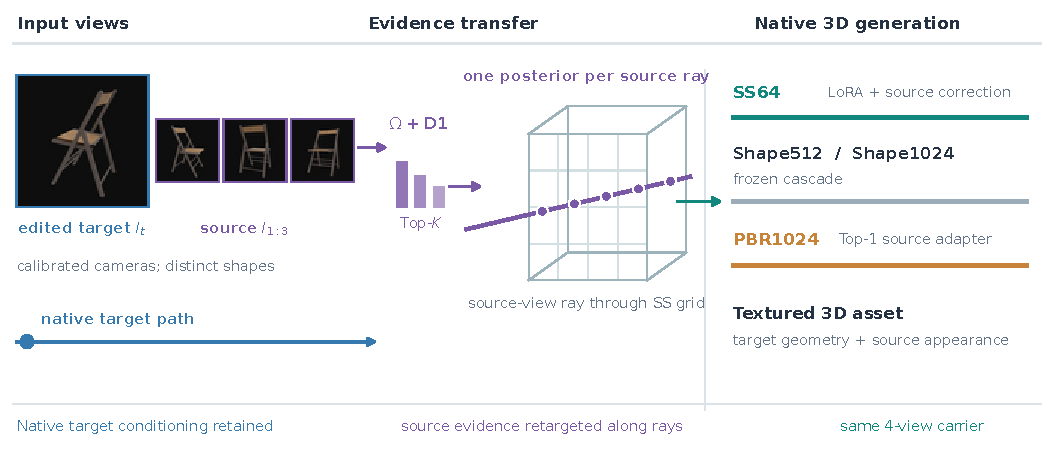
\includegraphics[width=\textwidth]{final-results/figures/paper-overall.pdf}
\caption{Stage-level overview. The edited target follows the native Pixal3D
conditioning path. Semantic evidence from undeformed source views corrects
the SS geometry carrier; Shape512/1024 are frozen. PBR uses a separately
selected Top-1 source retargeter for appearance. Figures~\ref{fig:matching}
and~\ref{fig:retargeting} explain the correspondence and source correction.}
\label{fig:selected-pipeline}
\end{figure*}

\subsection{Native carrier and the sharing unit}
Let $T$ be the target feature map, $S_j$ a source map, and $P_j$ its calibrated
bilinear projection. We retain the native four-view carrier
$C_{\mathrm{MV4}}$, including its target contribution and global tokens.
For source camera $j$ and image patch $p$, the sharing unit is
\begin{equation}
 \mathcal R_{j,p}=\{x:\pi_j(x)=p\}.
\end{equation}
Grid sites on this camera ray share an image-space evidence decision. The
decision is not an independently learned attention output for each voxel
feature. The SS implementation uses a $16^3$ conditioning grid and a
$32\times32$ patch map; SS64 denotes decoded occupancy resolution. Camera
projection defines membership without target surface depth or a
surface-visibility write mask at inference.

\subsection{Semantic proposals and matching scores}
\begin{figure}[t]
\centering
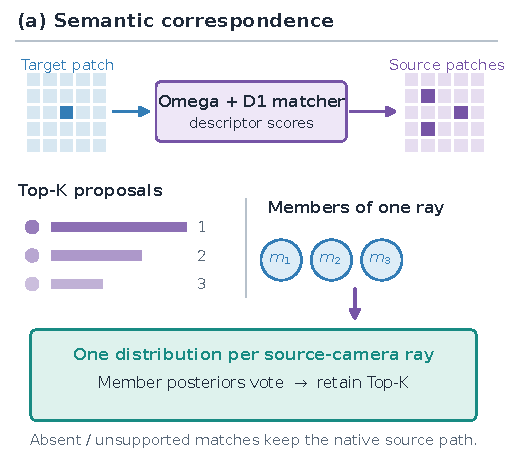
\includegraphics[width=\columnwidth]{final-results/figures/paper-matching.pdf}
\caption{Frozen semantic correspondence. Omega descriptors generate source
proposals and the D1 decoder scores them. Distinct observed target patches
sharing a source-camera ray vote into one Top-K posterior. Matching keys are
separate from the native source values used for generation.}
\label{fig:matching}
\end{figure}
Each observed target patch $m$ retrieves 64 semantic proposals across the
three source images. A frozen D1 decoder contextualizes its descriptor and
produces scores $s_{mk}$. The decoder has one query-only cross-attention block
and a bounded scalar residual head. Matching keys are 1024-dimensional
layer-12 FRAME Omega descriptors; SS values are separate, 1024-dimensional
native DINOv3 features.

Topology-derived barycentric correspondence and training-only depth checks
provide valid positive patch IDs $\mathcal P_m$. Given raw proposals
$\mathcal C_m$, the decoder minimizes
\begin{equation}
 \ell_m=-\log\frac{\sum_{k\in\mathcal C_m\cap\mathcal P_m}e^{s_{mk}}}
                       {\sum_{k\in\mathcal C_m}e^{s_{mk}}}.
\end{equation}
Only queries with a positive proposal contribute. Proposal misses and
unobservable queries are recorded separately. Decoder training uses 9,143
certified training examples and seven passes; Omega and the complete matcher
are frozen during subsequent generative fine-tuning. Topology/depth labels
are supervision and scoring data, not inference conditioning.

Distinct observed target patches in a source ray form its member set
$\mathcal M_r$. Their normalized distributions vote once per member:
\begin{align}
 \bar p_r(k)&=|\mathcal M_r|^{-1}\sum_{m\in\mathcal M_r}p_m(k),\\
 \mathcal K_r&=\operatorname{Top64}(\bar p_r),\qquad
 p_r(k)=\frac{\bar p_r(k)}{\sum_{l\in\mathcal K_r}\bar p_r(l)}.
\end{align}
Missing member entries have zero mass. Scores use softmax temperature 0.05.
This retains complementary modes before truncation instead of matching one
averaged descriptor. Input alpha and camera addresses define observation
support; they are not surface co-visibility. Empty members or insufficient
valid proposals abstain. A concentrated $p_r$ need not be correct: native
fallback detects missing support, not every confident mismatch.

\subsection{Matching-aware aggregation and retargeting}
\begin{figure}[t]
\centering
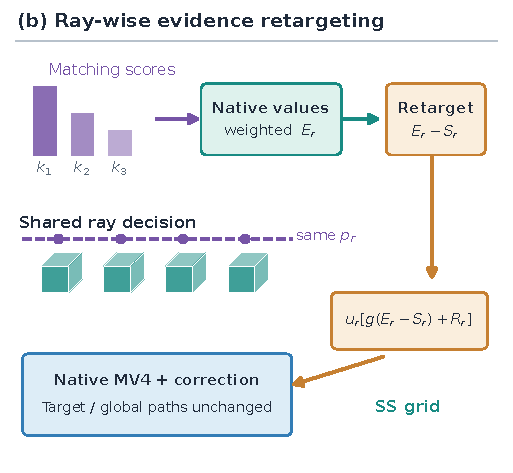
\includegraphics[width=\columnwidth]{final-results/figures/paper-retargeting.pdf}
\caption{One source-camera ray shares its posterior across intersected grid
sites. The selected SS path weights native source values, forms a bounded
source-contrast correction, and adds that correction to the native MV4
carrier. The target contribution and global tokens remain in the carrier;
unsupported rays retain the native source path.}
\label{fig:retargeting}
\end{figure}
The selected SS stage aggregates untransformed native values,
\begin{equation}
 E_r=\sum_{k\in\mathcal K_r}p_r(k)v_k.
\end{equation}
Carrier correction, source use, and retargeting consume this same evidence.
No additional learned Q/K or V/output head is required by this instantiated
design. Such heads are evaluated as alternatives, not declared necessary.

With learned source-use probability $u_r$ and signed bounded gate $g$,
\begin{align}
 R_r&=R_\phi([E_r-S_r,T_r]),\\
 \Delta_r&=u_r\{g(E_r-S_r)+R_r\},\\
 C&=C_{\mathrm{MV4}}+\tfrac14\sum_{j=1}^{3}P_j(\Delta_j).
\end{align}
$T_r$ pools native target context over the ray's grid sites; the distinct
observed members construct the matching distribution. Subtracting $S_r$
accounts for its existing contribution to the carrier. Initially $g=0$ and
the retargeter output is zero, recovering native conditioning. Unsupported
rays retain native source features rather than receive invented zero-valued
observations. Target feature extraction and its direct conditioning path are
retained, but exact generated target RGB preservation is not guaranteed.

\subsection{Stage-specific composition}
SS64 and PBR1024 continue their supplied multi-view LoRA checkpoints;
Shape512/1024 stay frozen. SS uses the weighted Fixed evidence above. The
selected appearance stage uses its separate Top-1 retargeter on generated
geometry. Its values are native DINOv3/NAF features. Neither the PBR feature
variants nor the SS learned-refinement variants are silently substituted for
this selected composition. Stage choices are based on their respective
geometric and fixed-geometry appearance development comparisons.
